\documentclass[../main.tex]{subfiles}
\begin{document}
在物理学当中,我们考虑任何问题之前,先假定了物理事件所发生的时空的几何结构。在本讲义中,我们假定物理事件发生的空间和时间是独立的。在这里我们先讨论空间的几何结构,它是3维欧几里得空间$\mathcal{E}$。

考虑任何一个具体的物理问题,都需要区分“系统”与“环境”。在连续介质力学中我们把“系统”称为\emph{物体(body)}。它在给定的某时刻$t$下在3维欧几里得空间中占据一个确定的区域$\Omega_t\subset\mathcal{E}$。我们称$\Omega_t$是物体的空间区域。在$\Omega_t$上,我们可以定义一个\emph{场(field)},它是一个函数$f:\Omega\rightarrow\mathcal{V}_f$。在物理学中,场的值是这个物体的某个强度性质在时刻$t$下的值,例如密度、速度、应力等。我们把物理量的值视为实数域上的内积空间$\mathcal{V}_f$的元素,是为了保持物理客观性,将在下面的讨论中详细说明。

作为欧几里得空间,$\mathcal{E}$有其附带的平移空间$\mathcal{V}_\mathcal{E}$。想要$\mathcal{E}$中的点$X\in \mathcal{E}$能唯一对应一个坐标$\left(x_1,x_2,x_3\right)\in\mathbb{R}^3$,需要选定一套坐标系。在之前的介绍中我们说过,任一欧几里得空间,自带一套直角坐标系$\left(O,\left\{\mathbf{\hat{e}}_i\right\}\right)$其中$O\in\mathcal{E}$,$\left\{\mathbf{\hat{e}}_i\right\}\subset\mathcal{V}_\mathcal{E}$。但是,我们也可以为欧几里得空间选取任一曲线坐标系,使得任一$X\in\mathcal{E}$仍然唯一地与一个$\mathbb{R}^3$的元素$\left(u_1,u_2,u_3\right)$对应。3维欧几里得空间中常见的两个曲线坐标系是\emph{柱坐标系(cylindrical coordinate)}和\emph{球坐标系(spherical coordinate)}。我们已经学过这两个坐标系的定义,这里不再赘述。场被一般地定义为$\mathcal{E}$上的函数,因此场的自变量是不依赖于坐标系的选择的。至于场函数的取值,作为内积空间$\mathcal{V}_f$中的一个向量,它应该具有基变换下的不变性。在物理学当中,大部分物理量的定义是通过空间和时间作出的,因此我们可以把$\mathcal{V}_f$的基变换问题归结为$\mathcal{E}$的基变换问题。从而,整个场的定义方式,就具有不依赖于坐标系的选择的不变性。用场来描述的物理事实,因此也就具有不依赖不同观察者坐标系选择的不变性。

我们具体讨论不同物理量体现在$\mathcal{V}_f$的维数。我们将看到,在我们所讨论的时空中的物理量取值只会是$3^n$维的,$n=0,1,2,\cdots$。

当$n=0$,我们称这样的物理量是一个\emph{标量场(scalar field)}。例如,温度场、密度场、压强场等。当$n=1$时,我们称这样的物理量是一个\emph{向量场(vector field)}。例如,速度场、位移场、力场等。当$n=2$时,我们称这样的物理量是一个\emph{二阶张量场(second-order tensor field)}。例如,应力场、应变场等。当$n=3$时,我们称这样的物理量是一个三阶张量场。当$n>3$时,我们称这样的物理量是一个高阶张量场。

在这里,所谓的“$n$阶张量”可理解为$\mathcal{L}\left(\mathcal{V}_\mathcal{E},\mathcal{V}_f\right)$上的线性变换,连同其在曲线坐标系下的坐标变换规律,的一套数学结构。在不涉及曲线坐标系变换问题时,张量就是相应的线性变换。把线性变换称作张量,是强调它的坐标表示要遵守欧几里得空间下场函数的曲线坐标变换规律。2阶张量是把一个向量变成另一个向量的线性变换,3阶张量是把一个向量变成一个二阶张量的线性变换,4阶张量则是把一个二阶张量变成另一个二阶张量的线性变换……以此类推。在连续介质力学中,固体的弹性系数、液体的粘滞系数都是4阶张量。因为它们是联系应力和应变的“系数”,而应力和应变本身就是二阶张量。只是对于各向同性不可压缩的最理想情况,它们的分量都只有1个非零值,故可退化为标量值的剪切模量和剪切粘度。

只要选定了某个坐标系,无论是场的自变量还是场的值,都分别可对应为$\mathbb{R}^3$上的和$\mathbb{R}^{3^n}$上的元素,从而场函数的讨论可等价为由$\mathbb{R}^3$到$\mathbb{R}^{3^n}$的向量函数的讨论,回到本章前面介绍的数学知识。但是,无论是场函数的导数还是积分,都保持独立于不同坐标系选择的不变性。这里我们详细讨论场函数的导数,并引出更多场论的概念。

\begin{figure}[h]
    \centering
    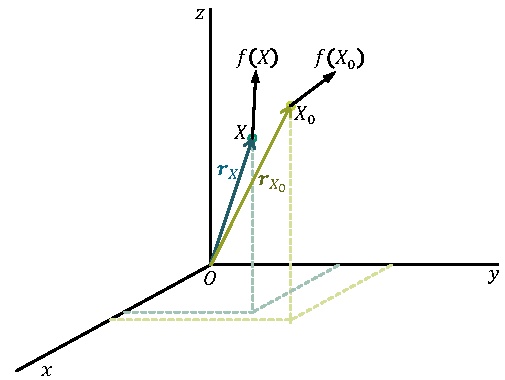
\includegraphics[width=0.75\textwidth]{images/vector_field_derivative.pdf}
    \caption{3维欧几里得空间中的向量场$f$在点$X$、$X_0$处的值,作为平移向量作在相应的点处(黑色箭头)。点$X$、$X_0$的位置向量是$\mathbf{r}_X$和$\mathbf{r}_{X_0}$。曲线$\mathcal{C}$过点$X$、$X_0$,向量场$f\left(X\right)$在曲线上的总作用要通过曲线积分求算(见\S\ref{sec:II.5.4})。}
    \label{fig:II.5.1}
\end{figure}

设$\mathcal{E}$是3维欧几里得空间,$\mathcal{V}_f$是一个实数域上的$3^n$维内积空间,函数$f:\mathcal{E}\supset\Omega_t\rightarrow\mathcal{V}_f$是某物体在$t$时刻某物理性质在其空间区域$\Omega_t$的场。所谓函数$f$在点$X_0\in\mathcal{E}$处可微分,即存在一个线性变换$\mathrm{D}f\left(X_0\right)\in\mathcal{L}\left(\mathcal{V}_\mathcal{E},\mathcal{V}_f\right)$满足:
\[\lim_{\left\|X-X_0\right\|\to 0}\frac{f\left(X\right)-f\left(X_0\right)-\mathrm{D}f\left(X_0\right)\left(X-X_0\right)}{\left\|X-X_0\right\|}=0\]
这里$\mathrm{D}f\left(X_0\right)$是该物体的性质$f$在$t$时刻下在空间位置点$X_0$处的导数。图\ref{fig:II.5.1}展示了$n=1$的例子。我们注意到,两个$\mathcal{E}$的点“相减”表示由一点到另一点的平移向量,故上式的意义是明确的。一旦选定了$\mathcal{E}$上的坐标系(包括曲线坐标系),则$\mathrm{D}f\left(X_0\right)$唯一对应一个$3^n\times 3$的矩阵,可称为场$f$在点$X_0$处的雅可比矩阵。这个矩阵是依赖坐标系(包括曲线坐标系)的选择的,但却不影响场的导数$\mathrm{D}f\left(X_0\right)$这一概念的独立性。诚然,如果场本身是表示客观的物理事实的,那么场的导数作为相应的物理性质的某种的空间变化率,也应是一个客观的物理事实,不应依赖于某观察者的坐标系选择。既然场的导数是一个不依赖坐标系(包括曲线坐标系)的线性变换,那么它的坐标矩阵必然要满足曲线坐标系的坐标变换规律,因此$n$张量场的导数是一个$n+1$阶张量。具体地,标量场的导数是一个向量场,向量场的导数是一个二阶张量场,二阶张量场的导数是一个三阶张量场,……以此类推。向量函数的梯度是其导数的转置,对于场函数的情况下也可类似地定义。我们照样可以记
\[\nabla f\left(X_0\right)=\left(\mathrm{D}f\left(X_0\right)\right)^\intercal\]
为场$f$在$X_0$处的\emph{梯度},或说物体的性质$f$在$t$时刻下在空间位置$X_0$处的梯度。梯度也具有坐标系选择的不变性。

对场的导数的分析,使用的无非是我们在前面所介绍过的对线性变换的分析方法。例如其行列式就是场的雅可比行列式,其迹就是场的散度,其斜称分量就是场的旋度,我们将在后面中详细讨论。
\end{document}


